\section{Risultati sperimantali}
\subsection{Prima parte - confronto con FFT}
Per confrontare l'efficienza computazionale tra la nostra implementazione della DCT2/IDCT2 e quella fornita dalla libreria \texttt{scipy}, è stato condotto un benchmark su matrici quadrate di dimensioni crescenti (da $32 \times 32$ fino a $8192 \times 8192$).
\newline
Per ciascuna dimensione:
\begin{itemize}
\item È stata generata una matrice casuale con valori reali in $[0,1]$.
\item È stata applicata la trasformata discreta del coseno bidimensionale (DCT2), seguita dalla cancellazione dei coefficienti ad alta frequenza (azzeramento del blocco in basso a destra della matrice trasformata).
\item È stata poi applicata la trasformata inversa (IDCT2).
\item Il tempo di esecuzione complessivo per DCT2 + IDCT2 è stato misurato con \texttt{time.perf\_counter()}.
\end{itemize}

Il processo è stato ripetuto sia con l’implementazione basata su \texttt{scipy.fftpack} (con normalizzazione \texttt{"ortho"}), sia con l’implementazione sviluppata manualmente, basata su prodotto matriciale e precomputazione della base DCT. \\

I tempi ottenuti sono stati registrati separatamente per ciascun approccio, consentendo un confronto diretto delle prestazioni al variare della dimensione della matrice, e i risultati temporali sono stati riportati su un grafico in scala semilogaritmica (ascisse lineari, ordinate logaritmiche).
Come atteso, l’implementazione manuale presenta una complessità computazionale dell’ordine di \( O(N^2) \), mentre la versione fornita dalla libreria è più efficiente, con una complessità stimata in \( O(N^2 \log N) \).

\begin{figure}[H]
    \centering
    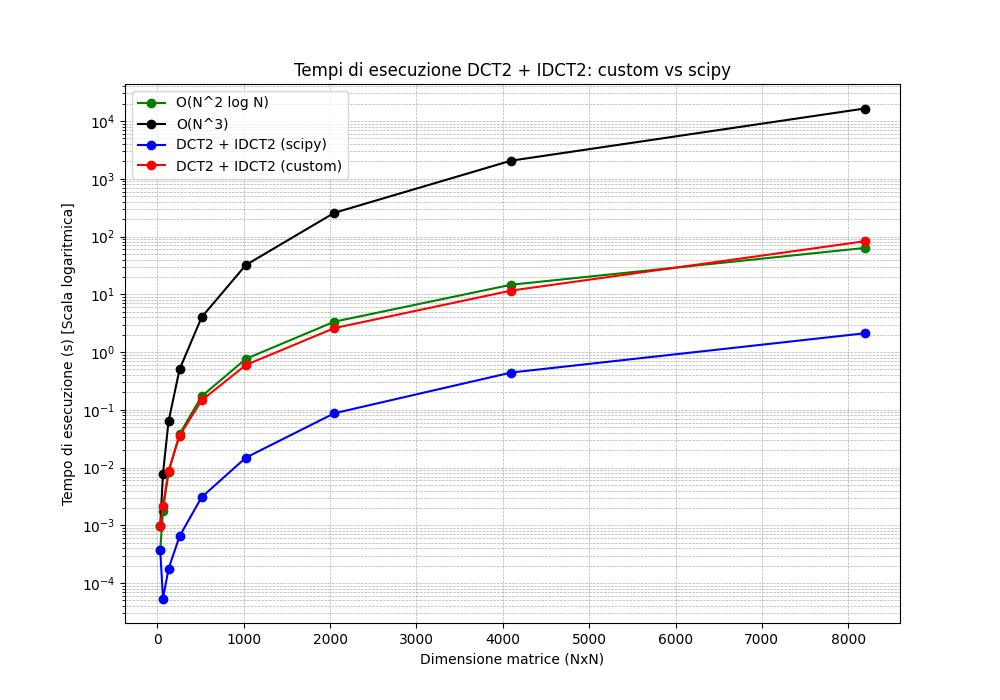
\includegraphics[width=0.9\textwidth]{images/benchmark.jpeg}
    \caption{Confronto tra i tempi di esecuzione della DCT2 implementata manualmente e quella fornita dalla libreria \texttt{scipy}.}
    \label{fig:benchmark}
\end{figure}

L’andamento dei tempi misurati è coerente con le complessità teoriche: per dimensioni moderate (\( N \approx 1000 \)) le differenze tra i due approcci sono già significative, e tendono ad aumentare all’aumentare di \( N \). Inoltre, l’implementazione ottimizzata mostra un comportamento più stabile e tempi sensibilmente inferiori in tutti i test effettuati, a conferma dell’efficienza dell’approccio basato su FFT per il calcolo della DCT2.

Questo confronto evidenzia l’importanza delle ottimizzazioni algoritmiche nei problemi numerici ad alta complessità, soprattutto quando si lavora con immagini di grandi dimensioni.

